%% ID: newtoniii
%% VIDEOS: newtoniii_sup.mp4
%% QUESTIONS: launching_a_rocket
%% CONCEPTS: newtoni, newtonii, vectors, calculus
%% LEVEL: 2
%% TOPIC: mechanics/dynamics
%% TYPE: physics
%% TITLE: Newton's Third Law
%% ORDER: 30
% This is the template that sets out all of the Problems and produces the Exercise/Solution labels and numbering
% There are two classes of Exercise: "problem" which has a Question and Solution, and "hint" which has a Question, Hint and Solution

% This is the template that sets out all of the Problems and produces the Exercise/Solution labels and numbering
% There are two classes of Exercise: "problem" which has a Question and Solution, and "hint" which has a Question, Hint and Solution

% These are the packages to use in all documents, and the paper size to use:
\documentclass[a4paper,11pt]{article}
\usepackage[usenames,dvipsnames]{xcolor}
\usepackage[margin=1.5cm]{geometry}
\usepackage{amsmath}
\usepackage{amssymb}
\usepackage{color}
\usepackage{graphicx}
\usepackage{graphics}
\usepackage[margin=1.5cm]{geometry}
\usepackage{fancyhdr}
\usepackage{float}
\usepackage{lscape}
\usepackage[font={small},labelfont=bf]{caption}
\usepackage{ifthen}
\usepackage{enumitem}
\usepackage{subcaption}		%Allows grouped figures. The percentage sign after the first \end{subfigure} puts them side by side, omitting it puts one above the other.
\usepackage{graphicx,xcolor} 	%Allows the use of colour in the files
\usepackage{centernot} 		%Puts the / in a not equal to sign in the centre, use as \cnot{...}
\usepackage{comment} 		%Allows \begin{comment} .... \end{comment} to comment out bulk text.
\usepackage{etoolbox}		%Allows the boolean flags and the \toggletrue and \togglefalse commands
\usepackage{cancel}		%Allows the crossing out of terms in maths mode to show they cancel out
\usepackage{wrapfig}

%Packages for font choices
\usepackage{palatino}
\usepackage{mathpazo}


%Then where to find the graphics:
%WARNING -  relative to the TeX file being compiled - NOT this template!
		\graphicspath{{../Diagrams/}{Diagrams/}{./}} %This allows diagrams: {{As a sister folder to Latex}{A subdirectory of LaTeX}{Or just in LaTeX itself}}

% WARNING -  If you want the diagrams to be a sister folder to the LaTeX folder - pdflatex.exe sometimes needs an extra argument to cope with the "../" part; usually it can only cope with subdirectories as opposed to parent ones. If it refuses to compile and says it cannot find the diagrams, either add "--shell-escape" to the start of the arguments of pdflatex, OR move the diagrams to a subdirectory of the one containing the TeX files.
%In TeXworks, to add the extra argument, go to Edit -> Preferences -> Typesetting -> Processing Tools. Click on "pdfLaTeX" -> Edit -> "+" button, then type "--shell-escape" (without quotes) and press the up arrow twice so that it becomes top of the list.


%Then any custom commands written, along with shortcuts and variables:
% This document contains any custom commands, shortcuts and variables needed for the files to compile. It is called by "Problem_Template.tex" and so needs to be in the same directory.

%Defines vectors universally, for ease of editing and consistency.
\newcommand{\vtr}[1] {\mathit{\underline{\boldsymbol{#1}}}}

%Draws a big red box containing the text as in \ALERT{<TEXT HERE>}. For labelling draft copies with important notes.
\def\ALERT#1{\begin{center}\colorbox{red}{\hbox{\textcolor{black}{\textbf{#1}}}}\end{center}}

%Roman-style subscript; removes math-mode font.
\def\s#1{_\textrm{#1} }

%The operators in integrals and derivatives.
\def\d{\operatorname{d}\!}

%The Euler e should be in Roman font.
\def\e{\textrm{e}}

%The Rutherford title, to save typing and for consistency:
\def\Rutherford{Rutherford School Physics}
\def\Concepttitle#1{\noindent\textsc{\Rutherford\vspace{0.4cm}\\ \LARGE Physical Concept: \textbf{#1}}}
\def\Problemtitle#1{\noindent\textsc{\Rutherford\vspace{0.4cm}\\ \LARGE Website Problems: \textbf{#1}}}
\def\AddProblemtitle#1{\noindent\textsc{\Large \Rutherford ~ --- ~ Additional Problems\vspace{0.4cm}\\ \LARGE \textbf{#1}}}
%\def\AddProblemtitle#1{\noindent\textsc{\Rutherford\vspace{0.4cm}\\ \LARGE Additional Problems: \textbf{#1}}}

%define quick question to be used in eg concept sheet.
%\def\qq#2{#1}{\color{red}[#2]\color{black}}
\newcommand{\qq}[2]{\nl Quick Question:\hspace{1 mm} #1\color{red}\hspace{2 mm} Answer:\color{black}\hspace{1 mm}  #2}
\newcommand{\stress}[1]{\emph{#1}}

%%%%%%%%%%%   some definitions used in latexing the CQMP:
% fractions that are of right size in set equations
\def\half{{\textstyle \frac{1}{2}}}
\def\quarter{{\textstyle \frac{1}{4}}}
\def\third{{\textstyle \frac{1}{3}}}
\def\eighth{{\textstyle \frac{1}{8}}}

% obtain a new line
\def\nl{\hfil\break}
\def\nll{\\ \\ \noindent}



%creates numbered lists with a), then i.
\renewcommand{\theenumi}{\alph{enumi}}% first level are latin characters
\renewcommand{\labelenumi}{\theenumi)} %tells it to put a bracket after the character.
\renewcommand{\theenumii}{\roman{enumii}}%second level are little roman characters
\renewcommand{\labelenumii}{\theenumii.} %tells it to put a dot after the character
 % In a file called "Definitions.tex" in the same directory as this file.

%Define some boolean switches:
\newtoggle{solutions_only}	%Print only the solutions
\newtoggle{no_solutions}		%Don't print any solutions  (overridden by solutions_only)
\newtoggle{solutions_at_end}	%Print the solutions at end (overridden by solutions_only and no_solutions)
\newtoggle{no_credits}		%Don't print the credit arguments

%Use this to write a list of things needed to know for a section. It automatically won't print when "solutions_only" is on.
%Its only argument should be a list of things needed to know in "\item [....]" form
\newenvironment{knowledge}[1]{
\iftoggle{solutions_only}{}{It is assumed that students will be familiar with the following concepts:
\begin{itemize} #1 \end{itemize}
\vspace{0.5cm}}
}

%Allows the headings to be managed when not printing problems ect.
\newenvironment{Qsection}[1]{
%\iftoggle{solutions_only}{}{\section{#1}} %Don't output headings in the solutions(?)
\iftoggle{solutions_at_end}{\AtEndDocument{\section{#1}}}{}
\section{#1}
}

\newenvironment{Qsubsection}[1]{
%\iftoggle{solutions_only}{}{\subsection{#1}} %Don't output headings in the solutions(?)
\iftoggle{solutions_at_end}{\AtEndDocument{\subsection{#1}}}{}
\subsection{#1}
}

%Set the values of the boolean switches: Yes - "toggletrue", No - "togglefalse".
\togglefalse{solutions_only}	%	ONLY		Output only solutions? 
\togglefalse{no_solutions}		%	NONE		Don't output solutions at all? 
\togglefalse{solutions_at_end}	%	END		Output solutions at the end?
\togglefalse{no_credits}		%			Don't output the credit field
%All 8 cases have been tested; ONLY takes precedence, then NONE and finally END is lowest.


%##############################################################################################################
%											Then the bulk of the layout options:
%##############################################################################################################

\setlength{\topmargin}{-2cm}
%\setlength{\oddsidemargin}{0.5cm}
%\setlength{\evensidemargin}{0.5cm}


%##############################################################################################################


\newcounter{exercisenumber}%[chapter] %counter is set to zero when "chapter" appears
\def\theexercisenumber{\arabic{exercisenumber}}


\iftoggle{no_solutions}{}{ %Put a header at the end before the solutions, and reset the counter. Only if solutions are being printed AND at the end.
	\iftoggle{solutions_only}{}{
		\iftoggle{solutions_at_end}
			{\AtEndDocument{\newpage \part*{Solutions:} \setcounter{exercisenumber}{0} \setcounter{section}{0}}}{}
	}
}


%%%%%%%%%%%%%%%%%%%%%%%%%%%%%%%%%%%%%%%%%%%%%%%%%%%%%%%%%%%%%%%%%%%%%%%%%%%%%%%%%
%Creates \begin{problem}[label]{exercise_text}{source_text}{solution_text}\end{problem} command - the label argument is optional
%If put in, remember to put in [] brackets.  A label called label.ex will be generated.
\newenvironment{problem}[4][noref]{
 \refstepcounter{exercisenumber} %\refstepcounter allows you to reference to the exercise number
%
\iftoggle{solutions_only}{\hfil\break \textit{Solution}~\theexercisenumber:  #4}{ %If only solutions, just output solution.
	\noindent{\textit{Exercise}~\theexercisenumber:}
	\ifthenelse{\equal{#1}{noref}}{}{\label{#1.ex}} #2 %\vspace{0.3cm}
	\iftoggle{no_credits}{}{
			%\hfil\break {\small #3} \vspace{0.3cm} %This is the old line, replaced with the one below, without the ifthenelse statement; in case something goes wrong.
			\ifthenelse{\equal{#3}{}}{}{ {\tiny [#3]} \vspace{0.3cm}} %If the credit field is blank; don't bother printing it or the space for it.
	} %reference argument
%
	\iftoggle{no_solutions}{}{ %If the solutions aren't to be printed, do nothing.
		\iftoggle{solutions_at_end}
			{\AtEndDocument{\stepcounter{exercisenumber}\hfil\break \textit{Solution}~\theexercisenumber:  #4 \vspace{0.5cm}}} %If at the end: do this.
			{\hfil\break \textit{Solution}~\theexercisenumber:  #4} 	%Else leave in line as in TeX file.
	}
}

\vspace{0.2cm}}

%%%%%%%%%%%%%%%%%%%%%%%%%%%%%%%%%%%%%%%%%%%%%%%%%%%%%%%%%%%%%%%%%%%%%%%%%%%%%%%%%
%Creates \begin{hint}[label]{exercise_text}{hint_text}{source_text}{solution_text}\end{hint} command - the label argument is optional
%If put in, remember to put in [] brackets.  A label called label.ex will be generated.
\newenvironment{hint}[5][noref]{
 \refstepcounter{exercisenumber}
%
\iftoggle{solutions_only}{\hfil\break \textit{Solution}~\theexercisenumber:  #5}{  %If only solutions, just output solution.
	\noindent{\textit{Exercise}~\theexercisenumber:}
	\ifthenelse{\equal{#1}{noref}}{}{\label{#1.ex}} #2 \vspace{0.1cm}
	 \hfil\break  \textit{Hint:}  #3{} %\vspace{0.3cm}
	\iftoggle{no_credits}{}{
			\ifthenelse{\equal{#4}{}}{}{\\ \hfil {\tiny #4} \vspace{0.3cm}} %This is the old line, replaced with the one below, without the ifthenelse statement; in case something goes wrong.
			%\ifthenelse{\equal{#4}{}}{}{{\tiny [#4]} \vspace{0.3cm}} %If the credit field is blank; don't bother printing it or the space for it.
	} %reference argument
%
	\iftoggle{no_solutions}{}{%If the solutions aren't to be printed, do nothing.
		\iftoggle{solutions_at_end}
			{\AtEndDocument{\stepcounter{exercisenumber}\hfil\break \textit{Solution}~\theexercisenumber:  #5 \vspace{0.5cm}}} %If at the end: do this.
			{\hfil\break \textit{Solution}~\theexercisenumber:  #5}%Else leave in line as in teX file.
	}
}
\vspace{0.2cm}}

%%%%%%%%%%%%%%%%%%%%%%%%%%%%%%%%%%%%%%%%%%%%%%%%%%%%%%%%%%%%%%%%%%%%%%%%%%%%%%%%%


 %%%%%%%
\newenvironment{additional}[2][noref]{
 \refstepcounter{exercisenumber}
% \vspace{.2cm}
\nl
\noindent{\textit{Exercise}~\theexercisenumber:}
\ifthenelse{\equal{#1}{noref}}{}{\label{#1.ex}} #2 }{%\vspace{5.1cm}
 }
%











%*******************************
% to mark as a draft.  Comment both these lines out when complete.  The page number will return to the footer.
%\pagestyle{myheadings}
%\markright{\textcolor{red}{\textbf{DRAFT: \today}}}


% It would be good if we could include my supervision video 2 as an example with this concept (just so that they can see what a "group" video might be like).

\begin{document}
\addtolength{\topmargin}{-0.7 cm}
\setlength{\columnsep}{22pt}
\Concepttitle{Newton's Third Law of Motion}

\begin{wrapfigure}{r}{8cm}\vspace{-1.5 cm}
\center
\includegraphics[width=0.35\textwidth]{../../figures/NewtonIII1.eps}
\caption{Free body force diagrams for a box on a table. Here \vari{W_b} is the weight of the box, \vari{N} is the normal reaction of the table on the box, \vari{W_t} is the weight of the table, and \vari{N_E} is the normal reaction of the Earth, or ground, on the table.} \label{NIII1}
\center
\includegraphics[width=0.35\textwidth]{../../figures/NewtonIII2.eps}
\caption{Free body force diagrams for a box on a table where we now include the Earth so that we can see the Newton pairs of the weights of the box and table.} \label{NIII2}
\end{wrapfigure}

\section{As Newton stated it...}
For every action (applied force) there is always an equal and opposite reaction (opposing force).


\section{Applying Newton III}
This law, as Newton stated it, does not always give us all the useful information that we might need.  What is implicit within this statement is that for every force there is an equal and opposite force of the \stress{same type}.  Let us take an example of a cardboard box on the table. \nl
In figure \ref{NIII1} we have drawn the free-body force diagram for the box and the table on which it sits.  If we look at the box alone we can make the mistake of pairing the normal force, \vari{N},  with the weight of box, \vari{W_b}.  The normal reaction and the weight are \stress{not} forces of the \stress{same type}. The weight of the box is due to the gravitational attraction of the box towards the Earth and the normal reaction (or contact force) is due to the electrostatic forces in the table pushing back on the box. To find a Newton pair of forces we need to look at the free-body diagram for the table \stress{and} the box. The force equal in size and opposite in direction to the normal reaction on the box (\vari{N} upwards) is the force of the box pushing atoms apart in the surface of the table (\vari{N} downwards).\nl
Newton's third law tells us that every force must have a pair so where are the pairs for the weight of the box, \vari{W_b}, the weight of the table, \vari{W_t}, and the normal reaction, \vari{N_E}? \  Figure \ref{NIII2} illustrates that to find the pairs for these forces we need to include the Earth.   \vari{W_b} and \vari{W_t} are the forces of gravitational attraction of the box and the table towards the Earth.  The Earth is attracted to the box (force pointing upwards from the Earth = \vari{W_b}) and the Earth is also attracted to the table (force pointing upwards from the Earth = \vari{W_t}).\nl
The force of gravitational attraction between the box and the table is another pair of forces that we could have added to this diagram but that force is so small that it is usually neglected (essentially zero).

\subsection{Level 4+}
Newton's Third Law allows us to consider large objects or systems of objects as composed of many smaller objects and we can then consider the free-body force diagrams for each component separately  often simplifying our calculations.\nl
\examp{Let us take the example of our box but this time we are going to consider the box as one large object of mass \vari{3m} and also as three small boxes of mass \vari{m} each (figure \ref{NIII3}).\nl  By combining Newton I with Newton III, calculate the value of all the reaction forces (\vari{N_1} to \vari{N_3}) for the stack of boxes in equilibrium on the right of figure \ref{NIII3} and show that the left and right diagrams are equivalent.}{\\ \valuedef{N_1-mg}{0}{}, \\
\valuedef{N_1+mg-N_2}{0}{},\\ \valuedef{N_2+mg-N_3}{0}{} therefore \nll
\valuedef{N_1}{mg}{,}  \valuedef{N_2}{2mg}{,} \valuedef{N_3}{3mg}{} and we can see that \valuedef{N_3}{N}{} (left diagram) as it should.}
\begin{wrapfigure}{r}{8cm}
\center
\includegraphics[width=0.35\textwidth]{../../figures/NewtonIII3.eps}
\caption{{\it Left:} The free body diagram of the forces acting on a cardboard box of mass, \vari{3m}, at rest on a table, where \vari{3mg} is weight of the box and \vari{N} is the normal reaction of the table on the box, \vari{W_t} is the weight of the table, and \vari{N_E} is the normal reaction of the ground on the table.\\
{\it Right:}  The free body diagram of the same cardboard box of mass, \vari{3m},  but this time cut in to three boxes of mass \vari{m} stacked on top of each other. } \label{NIII3}
\end{wrapfigure}



\end{document}
